\documentclass[paper=a4,
			   fontsize=12pt,
			   twocolumn=true
			   ]{scrartcl}
			   
\usepackage[latin1, utf8]{inputenc}
\usepackage[ngerman]{babel}
\usepackage{microtype}
\usepackage{geometry}
\usepackage{booktabs}
\usepackage{graphics}


\begin{document}
	
	\title{Überschiften müssen sein}
	\author{Hans Dampf \\ Dampfhammerstr. 1 \\ Eisenbahnhausen \\ h.dampf@tschutschubahn.de}
	
	\maketitle
	
	
	
%	\tableofcontents
	
	\section{Einleitung}
	
	Das ist unser erstes Dokument, bei dem wir in zwei Spalten schreiben, weil uns das so gut gefällt.
	
	Zunächst schreiben wir wie bei jedem Artikel eine Einleitung, weil sich das so gehört.
	
	Heute schreiben wir ein \LaTeX Dokument.
	
	\section{Hauptteil}
	
	Und weil sich das auch so gehört, schreiben wir einen langen Hauptteil. Hier sagen wir zwar nix, aber dafür reden wir um so mehr um den heißen Brei. Ist das nicht lustig?
	
	So, jetzt machen wir hier mal eine Aufzählung, in der nur heiße Luft ist:
	\begin{itemize}
		\item heiße Luft
		\item steigt auf
		\item und kühlt dabei ab
		\begin{itemize}
			\item stimmt das?
			\item tatsächlich?
		\end{itemize}
	\end{itemize}
	
	In so einen wissenschaftlichen Text muss natürlich mindestens eine Tabelle:\\

	
	\begin{table}
	\begin{tabular}{lcc}
			\toprule 
			Variable & Luft & Wasser \\
			\midrule
			Farbe & durchsichtig & blau\\
			Temperatur & kalt & heiß \\
			\bottomrule
			
		\end{tabular} \\
		\caption{eine tolle Tabelle!}
		\end{table}

	Und weil es grad so schön ist, führen wir für den Schmarrn noch eine Formel ein.
	
	Nicht zuletzt, wollen wir noch eine Abbildung einfügen. Die ist gleich hier
	
	\begin{figure}[h]
	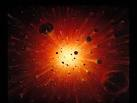
\includegraphics{Urknall.jpg}
	\caption{Urknall}
	\end{figure}

	
	
	\begin{equation}
	 \Delta = \frac{\xi^2}{\omega} 
	\end{equation}
	

	
	mit \( \Delta \) als Luft.
	
	 \section{Schluss}
	 
	 Auch das muss sein \footnote{totaler Schmarr, aber ok.}. Und wenn sie nicht gestorben sind, so leben sie noch heute \dots
	
\end{document}


